\documentclass[11pt]{article}
\usepackage{amsmath, amssymb, amsfonts}
\usepackage{geometry}
\usepackage{enumerate}
\usepackage{graphicx}
\usepackage{tikz}
\geometry{margin=1in}

\title{Backpropagation: Computing Gradients Efficiently\\
\large A Blackboard Teaching Guide}
\author{Based on Gilbert Strang's Linear Algebra and Learning from Data, Section VII.3}
\date{}

\begin{document}
\maketitle

\section{The Gradient Challenge in Deep Learning}

\subsection{Why We Need Efficient Gradients}
\textbf{The optimization problem:} Minimize loss $L(x)$ using gradient descent:
\begin{equation}
x_{k+1} = x_k - \alpha_k \nabla L(x_k)
\end{equation}

\textbf{In deep learning:}
\begin{itemize}
\item $x$ contains millions of parameters (weights and biases)
\item $L(x) = \frac{1}{N}\sum_{i=1}^N \ell(F(x, v_i), t_i)$ where $F(x,v)$ is our neural network
\item We need $\nabla L(x) = [\frac{\partial L}{\partial x_1}, \frac{\partial L}{\partial x_2}, \ldots, \frac{\partial L}{\partial x_M}]$
\item Computing this naively would be prohibitively expensive!
\end{itemize}

\textbf{The breakthrough:} Backpropagation computes all partial derivatives in roughly the same time as computing the function itself.

\section{Foundation: The Chain Rule}

\subsection{Single Variable Case}
For a composition $y = f_3(f_2(f_1(t)))$:
\begin{equation}
\frac{dy}{dt} = \frac{df_3}{df_2} \cdot \frac{df_2}{df_1} \cdot \frac{df_1}{dt}
\end{equation}

\textbf{Key insight:} We evaluate derivatives at the appropriate intermediate points.

\subsection{Multivariable Case}
For $F(x,y)$ depending on intermediate variables, if we have paths:
\begin{equation}
\frac{\partial F}{\partial x} = \sum_{\text{all paths from } x \text{ to } F} \left(\text{product of derivatives along path}\right)
\end{equation}

\section{Computational Graphs}

\subsection{Example: $F(x,y) = x^3(x + 3y)$}
Let's trace through with $x = 2, y = 3$.

\textbf{Forward computation:}
\begin{align}
\text{Step 1:} \quad c &= x^3 = 2^3 = 8\\
\text{Step 2:} \quad s &= x + 3y = 2 + 3(3) = 11\\
\text{Step 3:} \quad F &= c \cdot s = 8 \cdot 11 = 88
\end{align}

\textbf{Computational graph:}
\begin{center}
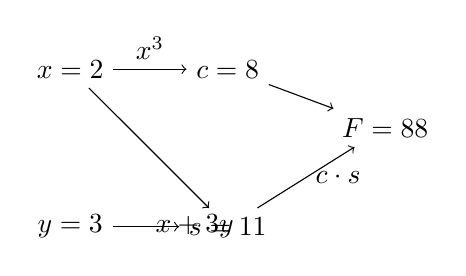
\begin{tikzpicture}[node distance=2cm]
\node (x) {$x=2$};
\node (y) [below of=x] {$y=3$};
\node (c) [right of=x] {$c=8$};
\node (s) [right of=y] {$s=11$};
\node (F) [right of=c, below=0.5cm] {$F=88$};

\draw[->] (x) -- (c) node[midway,above] {$x^3$};
\draw[->] (x) -- (s);
\draw[->] (y) -- (s) node[midway,right] {$x+3y$};
\draw[->] (c) -- (F);
\draw[->] (s) -- (F) node[midway,right] {$c \cdot s$};
\end{tikzpicture}
\end{center}

\section{Two Modes of Automatic Differentiation}

\subsection{Forward Mode: One Input at a Time}
\textbf{To compute $\frac{\partial F}{\partial x}$:}

\textbf{Step 1:} Compute intermediate derivatives:
\begin{align}
\frac{\partial c}{\partial x} &= 3x^2 = 3(2^2) = 12\\
\frac{\partial s}{\partial x} &= 1
\end{align}

\textbf{Step 2:} Apply product rule:
\begin{align}
\frac{\partial F}{\partial x} &= \frac{\partial F}{\partial c} \cdot \frac{\partial c}{\partial x} + \frac{\partial F}{\partial s} \cdot \frac{\partial s}{\partial x}\\
&= s \cdot 12 + c \cdot 1\\
&= 11 \cdot 12 + 8 \cdot 1 = 140
\end{align}

\textbf{Problem:} To get $\frac{\partial F}{\partial y}$, we need to repeat this entire process!

\textbf{Cost:} $M$ passes for $M$ input variables.

\subsection{Reverse Mode (Backpropagation): All Inputs at Once}
\textbf{Key idea:} Start from the output and work backwards.

\textbf{Step 1:} Initialize:
\begin{equation}
\frac{\partial F}{\partial F} = 1
\end{equation}

\textbf{Step 2:} Work backwards through each operation:
\begin{align}
\frac{\partial F}{\partial c} &= \frac{\partial F}{\partial F} \cdot \frac{\partial F}{\partial c} = 1 \cdot s = 11\\
\frac{\partial F}{\partial s} &= \frac{\partial F}{\partial F} \cdot \frac{\partial F}{\partial s} = 1 \cdot c = 8
\end{align}

\textbf{Step 3:} Continue backwards:
\begin{align}
\frac{\partial F}{\partial x} &= \frac{\partial F}{\partial c} \cdot \frac{\partial c}{\partial x} + \frac{\partial F}{\partial s} \cdot \frac{\partial s}{\partial x}\\
&= 11 \cdot 12 + 8 \cdot 1 = 140\\
\frac{\partial F}{\partial y} &= \frac{\partial F}{\partial c} \cdot \frac{\partial c}{\partial y} + \frac{\partial F}{\partial s} \cdot \frac{\partial s}{\partial y}\\
&= 11 \cdot 0 + 8 \cdot 3 = 24
\end{align}

\textbf{Amazing result:} We computed both partial derivatives in one backwards pass!

\section{Why Reverse Mode Wins: The Matrix Multiplication Analogy}

\subsection{The Three Matrix Problem}
Consider computing $ABC$ where:
\begin{itemize}
\item $A$ is $m \times n$
\item $B$ is $n \times p$ 
\item $C$ is $p \times q$
\end{itemize}

\textbf{Option 1: $(AB)C$}
\begin{itemize}
\item $AB$: $mnp$ operations
\item $(AB)C$: $mpq$ operations
\item Total: $mnp + mpq = mp(n + q)$
\end{itemize}

\textbf{Option 2: $A(BC)$}
\begin{itemize}
\item $BC$: $npq$ operations
\item $A(BC)$: $mnq$ operations  
\item Total: $npq + mnq = nq(m + p)$
\end{itemize}

\subsection{The Key Case: Column Vector}
\textbf{Suppose $C$ is a column vector ($q = 1$):}

\textbf{Option 1:} $mp(n + 1) \approx mpn$ operations

\textbf{Option 2:} $n(m + p)$ operations

\textbf{When $m, n, p$ are all large:} Option 2 is dramatically faster!

\subsection{Connection to Backpropagation}
\textbf{In neural networks, gradients have the form:}
\begin{equation}
\frac{\partial L}{\partial x} = \frac{\partial L}{\partial v_L} \cdot \frac{\partial v_L}{\partial v_{L-1}} \cdot \frac{\partial v_{L-1}}{\partial v_{L-2}} \cdots \frac{\partial v_1}{\partial x}
\end{equation}

\textbf{Key observation:}
\begin{itemize}
\item $\frac{\partial L}{\partial v_L}$ is like a "row vector" (few outputs)
\item $\frac{\partial v_1}{\partial x}$ is like multiplying by many columns (many weights)
\item Backpropagation = computing left-to-right (like $A(BC)$ with column $C$)
\item Forward mode = computing right-to-left (like $(AB)C$ - inefficient!)
\end{itemize}

\section{Backpropagation in Neural Networks}

\subsection{Layer Structure}
For layer $\ell$ with $N_{\ell-1}$ inputs and $N_\ell$ outputs:
\begin{align}
y_\ell &= A_\ell v_{\ell-1} + b_\ell\\
v_\ell &= \text{ReLU}(y_\ell)
\end{align}

\textbf{Matrix form with bias trick:}
\begin{equation}
M = \begin{bmatrix} 1 & 0^T \\ b & A \end{bmatrix}, \quad \begin{bmatrix} 1 \\ v \end{bmatrix} \rightarrow \begin{bmatrix} 1 \\ b + Av \end{bmatrix}
\end{equation}

\subsection{ReLU Derivatives}
\begin{equation}
\frac{d}{dz}\text{ReLU}(z) = \begin{cases}
1 & \text{if } z > 0\\
0 & \text{if } z < 0\\
\text{undefined} & \text{if } z = 0
\end{cases}
\end{equation}

\textbf{In practice:} We define the derivative at 0 to be 0 or 1 (doesn't matter much).

\subsection{The Backpropagation Algorithm}
\textbf{Forward pass:} Compute all $v_\ell$ and $y_\ell$ values.

\textbf{Backward pass:} For $\ell = L, L-1, \ldots, 1$:

\textbf{Step 1:} Compute gradient w.r.t. pre-activation:
\begin{equation}
\frac{\partial L}{\partial y_\ell} = \frac{\partial L}{\partial v_\ell} \odot \text{ReLU}'(y_\ell)
\end{equation}

\textbf{Step 2:} Compute gradients w.r.t. weights:
\begin{align}
\frac{\partial L}{\partial A_\ell} &= \frac{\partial L}{\partial y_\ell} v_{\ell-1}^T\\
\frac{\partial L}{\partial b_\ell} &= \frac{\partial L}{\partial y_\ell}
\end{align}

\textbf{Step 3:} Propagate to previous layer:
\begin{equation}
\frac{\partial L}{\partial v_{\ell-1}} = A_\ell^T \frac{\partial L}{\partial y_\ell}
\end{equation}

\section{Computational Efficiency}

\subsection{Cost Analysis}
\textbf{Forward pass:} Compute $F(x,v)$
\begin{itemize}
\item Dominated by matrix multiplications
\item Cost roughly proportional to number of weights
\end{itemize}

\textbf{Backward pass:} Compute all partial derivatives $\frac{\partial F}{\partial x_i}$
\begin{itemize}
\item Also dominated by matrix multiplications
\item Cost roughly 2-3 times the forward pass
\item Independent of the number of parameters!
\end{itemize}

\textbf{Magic:} Cost is $O(\text{forward pass})$, not $O(M \times \text{forward pass})$ where $M$ is the number of parameters.

\subsection{Why This Matters}
\textbf{Modern networks:}
\begin{itemize}
\item GPT-3: 175 billion parameters
\item Forward pass might take 1 second
\item Naive gradient: $175 \times 10^9$ seconds ≈ 5,500 years
\item Backpropagation: ~3 seconds
\end{itemize}

\section{Practical Implementation Details}

\subsection{Computational Graph Frameworks}
\textbf{Modern deep learning frameworks:}
\begin{itemize}
\item TensorFlow, PyTorch, JAX
\item Automatically build computational graphs
\item Automatic differentiation via backpropagation
\item Handle complex architectures (CNNs, RNNs, Transformers)
\end{itemize}

\subsection{Memory vs. Computation Trade-offs}
\textbf{Checkpointing:} Save only some intermediate values, recompute others
\begin{itemize}
\item Saves memory at cost of extra computation
\item Essential for very deep networks
\item Gradient checkpointing reduces memory from $O(L)$ to $O(\sqrt{L})$
\end{itemize}

\section{Advanced Topics}

\subsection{Higher-Order Derivatives}
\textbf{Hessian-vector products:} Can be computed efficiently using forward-mode AD applied to backpropagation.

\textbf{Applications:}
\begin{itemize}
\item Second-order optimization methods
\item Uncertainty quantification
\item Model analysis
\end{itemize}

\subsection{Numerical Stability}
\textbf{Vanishing gradients:} Products of many small derivatives
\begin{itemize}
\item Problem in very deep networks
\item Solutions: Skip connections, normalization, careful initialization
\end{itemize}

\textbf{Exploding gradients:} Products of many large derivatives
\begin{itemize}
\item Can cause training instability
\item Solution: Gradient clipping
\end{itemize}

\section{The Complete Picture: SGD + Backpropagation}

\subsection{The Training Loop}
\textbf{For each epoch:}
\begin{enumerate}
\item \textbf{Forward pass:} Compute $F(x_k, v_i)$ for minibatch
\item \textbf{Loss computation:} Compute $\ell(F(x_k, v_i), t_i)$
\item \textbf{Backward pass:} Compute $\nabla_x \ell$ via backpropagation
\item \textbf{Parameter update:} $x_{k+1} = x_k - \alpha \nabla_x \ell$
\end{enumerate}

\subsection{Why This Works}
\textbf{Mathematical foundation:}
\begin{itemize}
\item Chain rule guarantees correctness
\item Reverse mode ensures efficiency
\item SGD provides convergence (under appropriate conditions)
\end{itemize}

\textbf{Practical success:}
\begin{itemize}
\item Enables training of massive models
\item Foundation of modern AI breakthroughs
\item Scales to billions of parameters
\end{itemize}

\section{Summary}

\textbf{Key insights:}
\begin{enumerate}
\item \textbf{Computational graphs:} Visualize complex function composition
\item \textbf{Chain rule:} Mathematical foundation for automatic differentiation
\item \textbf{Reverse mode:} Efficient when many inputs, few outputs
\item \textbf{Matrix multiplication analogy:} Order matters enormously
\item \textbf{Practical impact:} Makes deep learning computationally feasible
\end{enumerate}

\textbf{The bottom line:} Backpropagation is not just a clever trick - it's the computational insight that makes modern deep learning possible. By organizing the chain rule computation in the right order, we can compute gradients efficiently regardless of the number of parameters.

\textbf{Next steps:} With efficient gradients in hand, we can explore advanced optimization methods, regularization techniques, and the art of training deep networks successfully.

\end{document}